\RequirePackage{etex}
\RequirePackage{easybmat}
\documentclass[10pt]{article}  % list options between brackets
\usepackage{etex}
%\usepackage[english]{babel} % Adatta LaTeX alle convenzioni tipografiche italiane
%\usepackage[utf8]{inputenc} % Consente l'uso dei caratteri accentati italiani
\usepackage{mdframed} %per mettere delle box attorno a qualsiasi cosa
\usepackage{graphicx} % Per le immagini
\usepackage {fancyhdr} % Per l' ambiente abstract
\usepackage{indentfirst} % Indentazione all' inizio dei capitoli
\usepackage{url} % Formattazione URL
\usepackage{amsmath} % Vari simboli matematici
\usepackage{amssymb} %Per l' "uguale per definizione"
\usepackage{amsthm} % Per le dimostrazioni
\usepackage{amsfonts} % Per font matematici
\usepackage{mathrsfs} % Per i font corsivi belli, tipo la N delle gaussiane ecc...
\usepackage{listings} % Per il codice
\usepackage{easybmat} % Per le matrici a blocchi
\usepackage{mathtools}
\usepackage{color}
\usepackage{tikz}
\usepackage{syntax}
\usetikzlibrary{trees}
\newcommand{\fncyblank}{\fancyhf{}} %
\frenchspacing % Non aumentare la spaziatura tra periodi
\newcommand{\footnoteremember}[2] % Accesso multiplo a note a pie' pagina
{
    \footnote{#2}
    \newcounter{#1}
    \setcounter{#1}
    {
        \value{footnote}
    }
}
\newcommand{\footnoterecall}[1]
{
    \footnotemark[\value{#1}]
}

\lstdefinelanguage{JavaScript}{
  keywords={typeof, new, true, false, catch, function, return, null, catch, switch, var, if, in, while, do, else, case, break},
  ndkeywords={class, export, boolean, throw, implements, import, this},
  sensitive=false,
  comment=[l]{//},
  morecomment=[s]{/*}{*/},
  morestring=[b]',
  morestring=[b]"
}

\begin{document}
\title{Advanced Programming\\final term paper}   % type title between braces
\author{Cosimo Sacco}         % type author(s) between braces
\date{}    % type date between braces
\maketitle
\begin{abstract}
    This paper describes the \emph{PAQL code generator}, a \emph{Java} and \emph{C++} project
    developed by the author in the frame of the
    \emph{Advanced Programming} academic course. \emph{PAQL} is an \emph{element}, \emph{container} and
    \emph{query} description language. The \emph{PAQL code generator} translates
    a \emph{PAQL description} into a suitable set of \emph{C++} classes simulating the \emph{LINQ C\# mechanism}.
\end{abstract}
\section{PAQL basic grammar}
    \label{sec:basicPAQL}
    \emph{PAQL} basic grammar $G_{PAQL}$:
    \vspace{1em}
    \begin{mdframed}
        \begin{grammar}
            <description> ::=
                <element> <description> | <container> <description> \alt <query> <description> | $\varepsilon$

            <element> ::=
                `element' <identifier> `{' <declarationBlock> `}'

            <declarationBlock> ::=
                <keyDeclaration> <declarationBlock> \alt `{' <varDeclarationBlock> `}'

            <keyDeclaration> ::=
                `key' `{' <varDeclarationBlock> `}'

            <varDeclarationBlock> ::=
                <variableDeclaration> <varDeclarationBlock> \alt $\varepsilon$

            <variableDeclaration> ::=
                <identifier> <identifier> `;'

            <container> ::=
                `container' `<' <identifier> `>' <identifier> `;'

            <query> ::=
                `query' `<' <identifier> `>' <identifier> `(' <identifier> `)' `;'
        \end{grammar}
    \end{mdframed}
    \vspace{1em}
    \emph{PAQL} parsing table:
    \begin{center}
    \begin{tabular}{ | c | c | c | c | c | c | c | c | c |}
        \hline
                           & $\mathbf\varepsilon$ & \textbf{identifier} & \textbf{query} & \textbf{container} & \textbf{\}} & \textbf{\{} & \textbf{key} & \textbf{element} \\
        \hline
\textbf{$\langle$description$\rangle$}& $a_3$ & & $a_2$              & $a_1$         &                &             &             & $a_0$\\
       \hline
\textbf{$\langle$element$\rangle$} & &                    &                &                    &             &             &              & $b$\\
        \hline
\textbf{$\langle$declarationBlock$\rangle$} & &                 &                &                    &            &  $c_1$       &  $c_0$    &\\
        \hline
\textbf{$\langle$keyDeclaration$\rangle$} & &               &                &                    &             &         &  $d$       &\\
        \hline
\textbf{$\langle$varDeclarationBlock$\rangle$} &  &  $e_0$               &                &                    &      $e_1$  &      &         &\\
        \hline
\textbf{$\langle$varDeclaration$\rangle$} &  &    $f$             &                &                    &             &        &         &\\
        \hline
\textbf{$\langle$container$\rangle$} & &               &                &              g      &             &         &         &\\
        \hline
\textbf{$\langle$query$\rangle$} & &                &         $h$       &                    &             &         &         &\\
        \hline
    \end{tabular}
    \end{center}
    Let $c_{i,j}$ be the cell of $P$ in the position $(i, j)$. Then
    \[
        \#(c_{i,j}) \in \left\{ 0, 1 \right\}\ \forall i,j : c_{i,j} \in P \implies G_{PAQL}\sim LL(1).
    \]
\section{Generated classes}
    \subsection{Element model class}
        The element model class is a simple struct which defines the \emph{equal to} operator as follows.
        \begin{lstlisting}[language=C++]
bool operator==(const Element& e) const
{
    return (e.v1 == v1) && ... && (e.vN == vN) && (true);
}
        \end{lstlisting}
        Where $v_i$ represents the $i$-th declared variable.
    \subsection{Container model class}
        This \emph{PAQL} implementation allows \emph{multiple superkeys with variable arity and composing types}.
        Each key is defined by a tuple of types. Also, different keys can be defined through the same \emph{type tuple}. An example:
        \begin{lstlisting}[language=C++]
key {int personalCode; string nation;}
key {int studentCode; string university;}
key {string username; string password;}
        \end{lstlisting}

        In order to provide an efficient container lookup, a \emph{map} should be provided
        for each defined key, and a proper \emph{get} method which uses the right map to find the result.
        The main problems to face in this case are three:
        \begin{enumerate}
            \item The \emph{key type} is a type tuple. How can a tuple of hetherogeneous types be managed?
            \item The generated methods \texttt{Element\& get(int personalCode, string nation)} and
            \texttt{Element\& get(int studentCode, string university)}
                would have the same signature, which is illegal. How can two key types whose type tuple is the same be distinguished?
            \item The \texttt{Element\& get(int personalCode, string nation)} and
            \texttt{Element\& get(int studentCode, string university)} methods should
            lookup on two different maps. How can a key type be linked to the proper map?
        \end{enumerate}
        Those problems are addressed through \emph{template metaprogramming} techniques.

        A container is implemented as the \emph{fusion} of a \emph{generic list} and a \emph{meta map\footnote{
        A \emph{meta map} is a map where the keys are types, and access is resolved at compile time.} of heterogeneous maps\footnote{We could refer
        to this structure as a $\mu\varepsilon\tau\alpha$ \emph{meta} \emph{map}, where $\mu\varepsilon\tau\alpha$ is referred to the fact that the map values are also maps, while \emph{meta} is referred to the fact that
        those values are accessed at compile time.}}
        through \emph{multiple virtual inheritance}
        from those structures\footnote{Implemented by \texttt{std::list} and \texttt{boost::fusion::map} respectively.}.
        The \emph{``list nature''} of the container allows general element access, while its \emph{``meta map nature''}
        conveys to fast access. Figure \ref{fig:containerUML} shows the type relations involved in each container class.
        \begin{figure}[htbp]
            \centering
            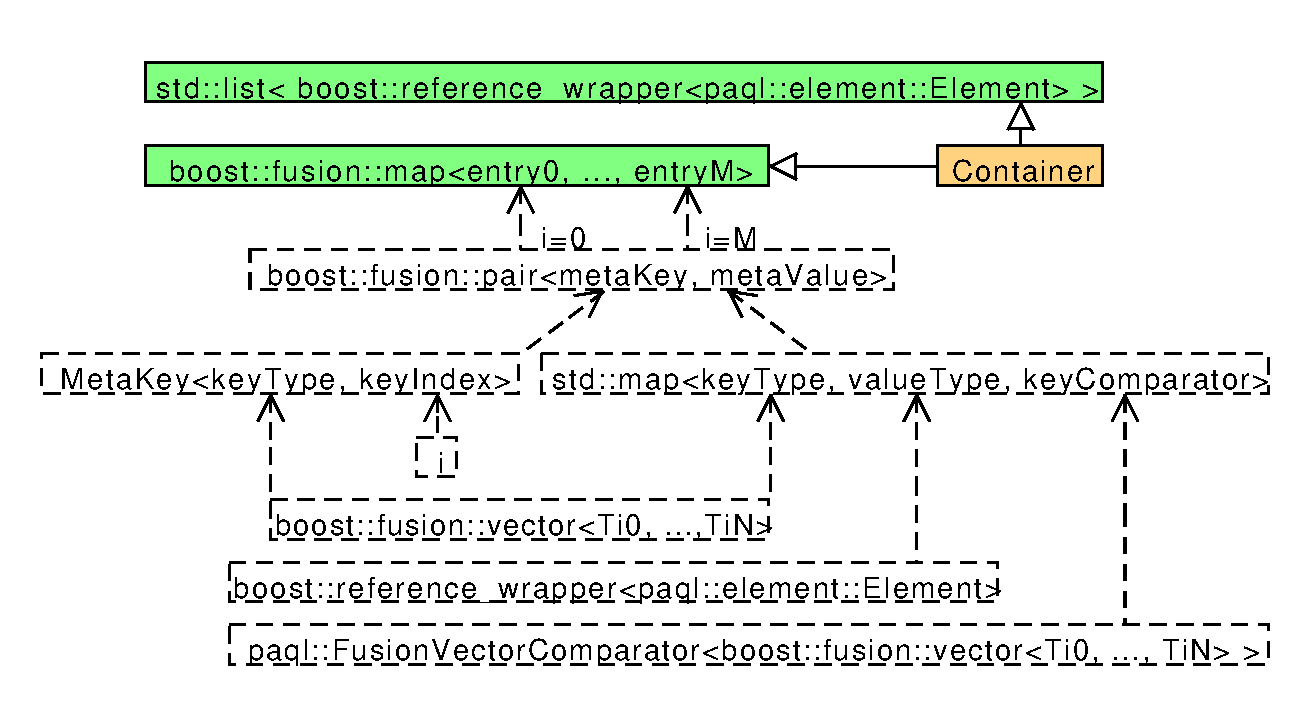
\includegraphics[scale=0.5]{Container.pdf}
            \caption{The container type genesis}\label{fig:containerUML}
        \end{figure}
        A \texttt{Container} is a \emph{list of references}\footnote{\texttt{boost::reference_wrapper} allows to pass references as template
        parameters.} to elements and a \emph{set of maps} which index the contained references
        according to each key definition. Each map is identified by its \emph{meta key}, which is a type, and is
        retrieved at compile time through the \emph{meta selection operator} \texttt{boost::fusion::at_key<keyType>}.
        The \emph{meta keys} are composed by the \emph{key type}, which is a \emph{type tuple} composed through the \emph{variadic
        template class} \texttt{boost::fusion::vector<T0, ..., TN>}, and its index, which is an integer constant.
        Each retrieved map is indexed by the related \emph{key type}, and refers the same objects contained
        in the references list.
        The operations defined on a container are:
        \begin{itemize}
            \item \textbf{insertion}: given an element to insert, a new entry is created in each map and gets indexed by
            the proper key (created using, each time, the proper element members) and the element reference is added to the list;
            \item \textbf{selection}: given a key of some type, a proper \emph{get} method is provided,
            which selects the element reference using the passed key in the right map;
            \item \textbf{removal}: given an element reference, the \emph{remove} to delete each entry
            related to that element in each map, and remove it from the list;
        \end{itemize}
    \subsection{Query model class}
        In the first, basic version of \emph{PAQL}, the generated query classes are very simple. The query execution
        method simply retrieves all the elements from its container instance \texttt{c} and returns the formed list.
        \begin{lstlisting}[language=C++]
std::list<boost::reference_wrapper<paql::element::Element> > execute()
{
    typedef
        std::list
        <
            boost::reference_wrapper
            <
                paql::element::Element
            >
        >
        List;
    List r;
    for
    (
        List::iterator i = c.begin();
        i != c.end();
        i++
    ) r.push_back((*i));
    return r;
}
        \end{lstlisting}
\section{Parsing and code generation}
    A \texttt{System} is an object which transforms a generic \emph{input} object into an \emph{output} object
    through its \texttt{transform(Input, Output)} method. A \texttt{Compiler} is a \texttt{System} which transforms an \texttt{InputStream}
    into a \texttt{List<SourceFile>}. A \texttt{Compiler} is made up of several sub\texttt{System}, linked in a \emph{pipeline} where
    each \emph{output} is an \emph{input} for the following. Each subsystem manages a particular phase of the compilation process,
    in particular
    \begin{itemize}
        \item \texttt{LexicalAnalyzer}: given an \emph{input stream}, it recognizes valid \emph{language tokens}, thus performing a
        \emph{lexical check}, and builds up a \emph{token list};
        \item \texttt{SyntacticAnalyzer}: given a \emph{list of valid tokens}, it recognizes valid \emph{syntactic structures}
        and represents them in the form of a \emph{parse tree}, thus performing a \emph{syntactic check};
        \item \texttt{SemanticAnalyzer}: given a valid \emph{parse tree}, it checks its semantic validity and builds up
        \emph{language specific semantic structures};
        \item \texttt{CodeGenerator}: given a valid \emph{semantic structure}, it serializes it to a \emph{list of source files}
        whose language is the \emph{object language};
    \end{itemize}
    Those interfaces are implemented to satisfy the \emph{PAQL} specifications, so the \emph{PAQL} compiler is built up by
    the systems of concrete classes \texttt{PAQLLexicalAnalyzer}, \texttt{PAQLSyntacticAnalyzer}, \texttt{PAQLSemanticAnalyzer} and
    \texttt{PAQLCodeGenerator}. Figure \ref{fig:compiler} shows the class hierarchy and relations.
    \begin{figure}[htbp]
    \hspace{-7em}
        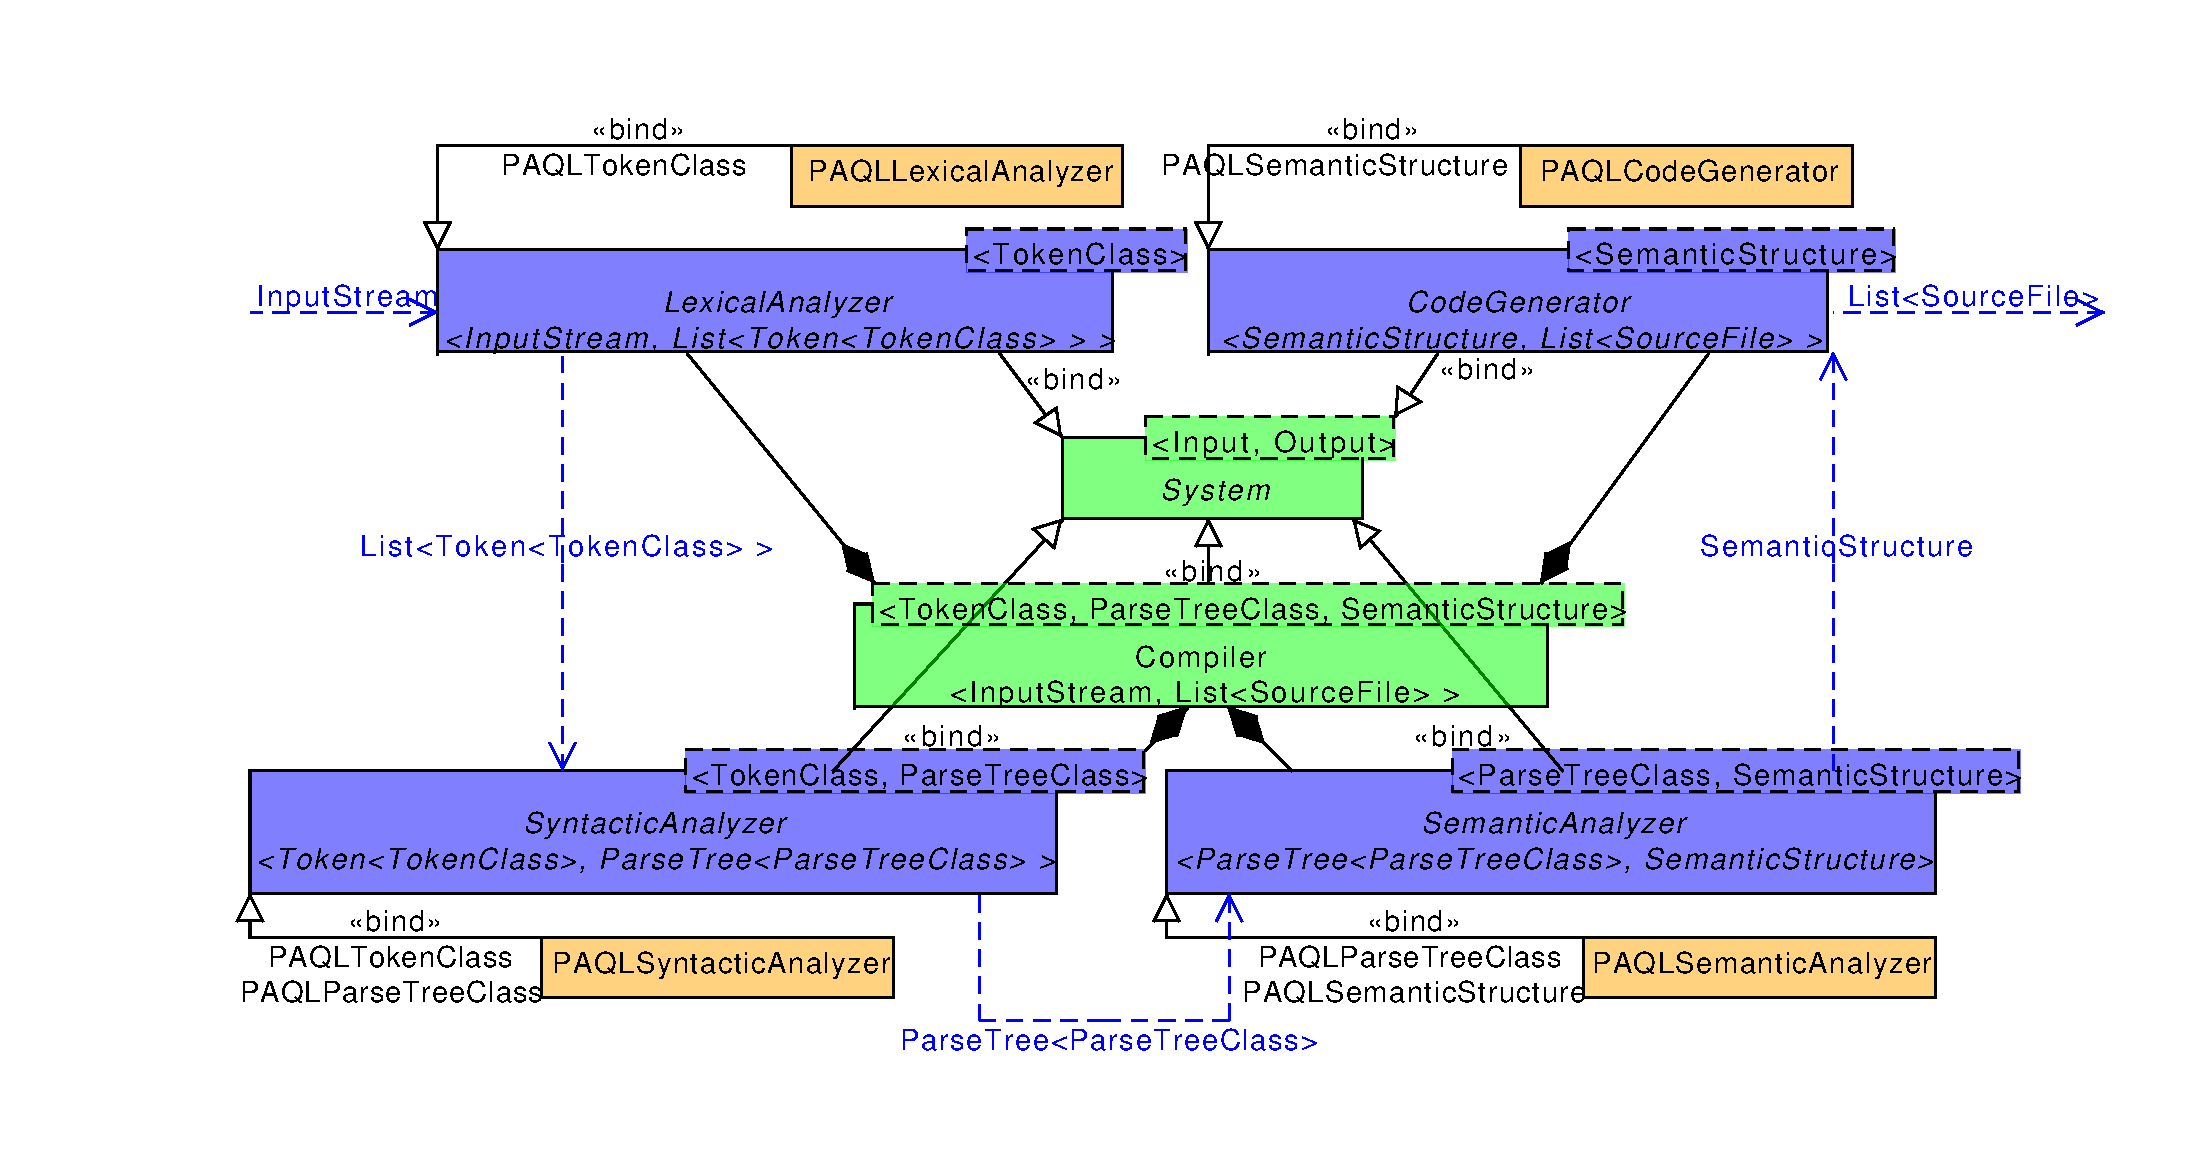
\includegraphics[scale=0.45]{Compiler.pdf}
        \caption{The \emph{PAQL} compiler classes}\label{fig:compiler}
    \end{figure}
    In particular, \texttt{PAQLSyntacticAnalyzer} is implemented as a \emph{recursive descent parser}, which offers a parse method
    for each syntactic cathegory:
    \begin{lstlisting}[language=Java]
// "typedef" ParseTree<PAQLParseTreeClass> PT;
// "typedef" Iterator< Token<PAQLTokenClass> > TI
private PT parseDescription(TI tokenIterator);
private PT parseElement(TI tokenIterator);
private PT parseDeclarationBlock(TI tokenIterator);
private PT parseKeyDeclaration(TI tokenIterator);
private PT parseVariableDeclarationBlock(TI tokenIterator);
private PT parseVariableDeclaration(TI tokenIterator);
private PT parseContainer(TI tokenIterator);
private PT parseQuery(TI tokenIterator);
        \end{lstlisting}
    \emph{Tokens}, \emph{parse trees}, \emph{semantic structures} and \emph{source files} are represented by dedicated classes.
    Figure \ref{fig:tokenandparsetree} shows the class hierarchy of tokens and parse trees. In particular, both \texttt{Token}
    and \texttt{ParseTree} are \texttt{MetaType}s. The \texttt{MetaType} interface allows to explicitly refer the \emph{intended}
    type of an object \emph{preventing} class proliferation and \emph{avoiding} the use of reflection. This result is obtained
    maintaining the type information as an enumerate, whose type can be defined according to the particular application. In this
    cases, the \texttt{PAQLTokenClass} and \texttt{PAQLParseTree} enumerates define the \emph{intended types} for tokens and parse trees.
    Using inheritance, particular tokens and parse trees are defined: an \texttt{EvaluableToken} is a \texttt{Token} which can be
    \emph{evaluated} (constants, identifiers\ldots), while a particular parse tree is defined for each \emph{PAQL} construct,
    and the \emph{aggregation relationships} reflect the \emph{PAQL grammar}.
    \begin{figure}[htbp]
        \centering
        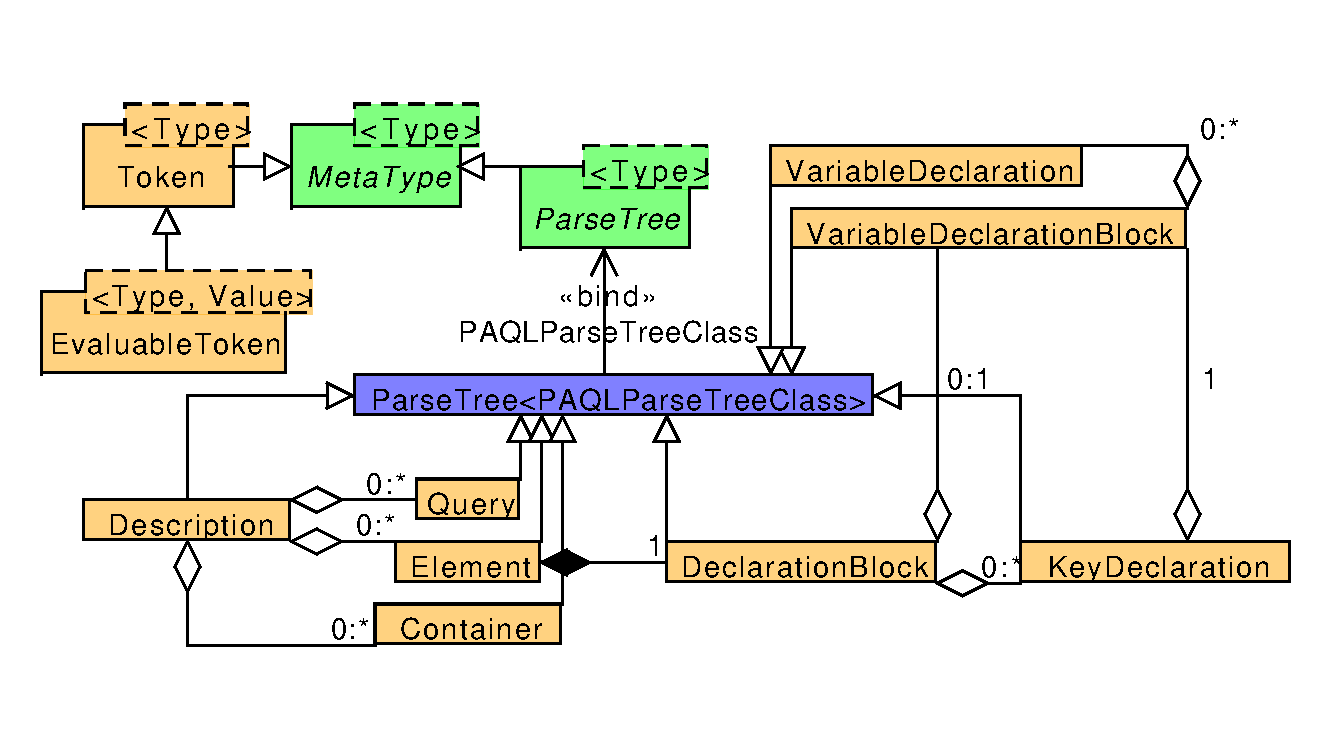
\includegraphics[scale=0.45]{classDIagram.pdf}
        \caption{The \emph{PAQL} \emph{token} and \emph{parse tree} class hierarchy }\label{fig:tokenandparsetree}
    \end{figure}

    The \emph{semantic structure} produced by a particular \texttt{CodeGenerator} is application specific. In the case of \emph{PAQL},
    this structure is described in figure \ref{fig:semanticStructure}.
    The \texttt{PAQLSemanticStructure} maintains informations about each declared \emph{element}, \emph{container} or \emph{query}.
    The formal properties of the \texttt{Set} (\emph{value uniqueness}) and \texttt{Map} (\emph{key-value uniqueness}) containers
    are exploited to enforce semantic consistency of declarations.
    The element informations are indexed in a map, whose key type is the declared element name.
    For each element, its variable set and keyset is maintained. In particular, the keyset is maintained in the form of a map indexed by the key index.
    The informations related to containers and queries are simpler, those are, respectively, \texttt{Pair} and \texttt{Triple} of type names.

    \texttt{SourceFile} is a simple string wrapper with serialization capabilities.
    \begin{figure}[htbp]
        \centering
        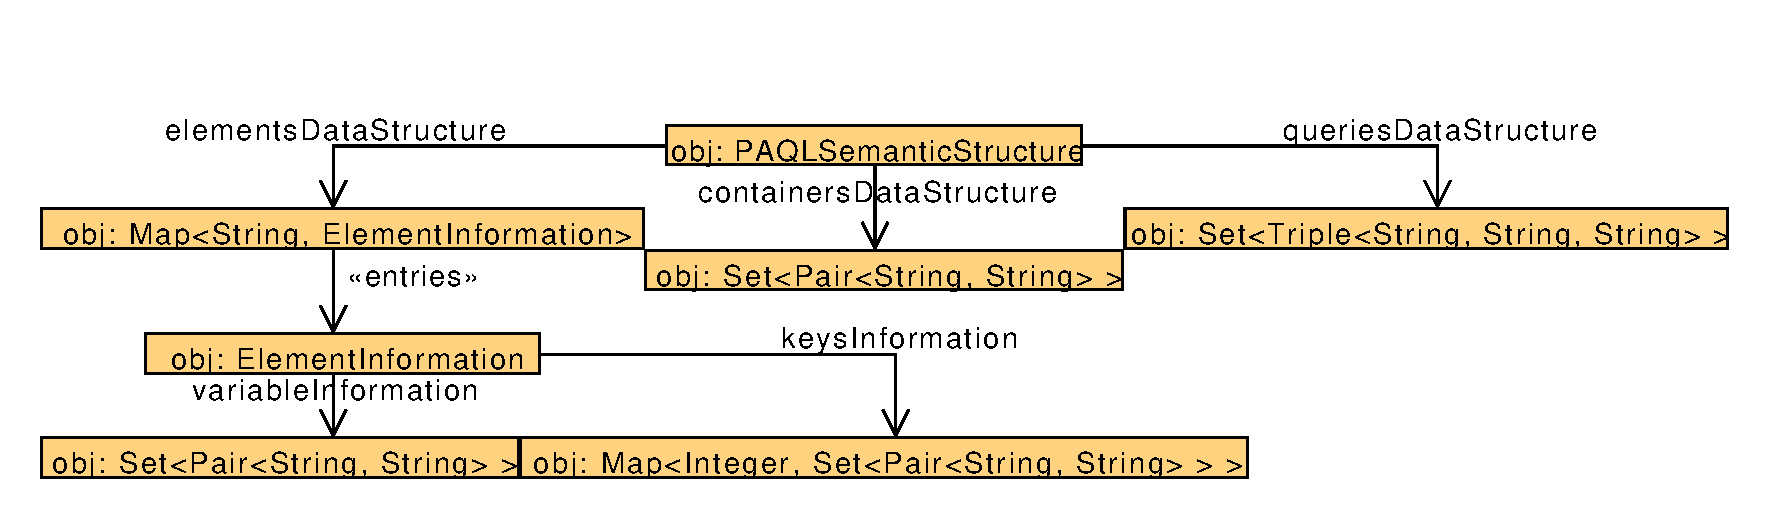
\includegraphics[scale=0.45]{semanticStructure.pdf}
        \caption{The \emph{PAQL semantic structure}}\label{fig:semanticStructure}
    \end{figure}
\section{Conditional queries}

    \begin{center}
        \textbf{\emph{Due to lack of time, this extension has not been implemented}}
    \end{center}

    The \emph{PAQL} grammar can be extended to allow \emph{conditional queries}, id est queries where the result is filtered by a condition
    on elements. The $\langle$\emph{query}$\rangle$ production is modified as follows:
    \vspace{1em}
    \begin{mdframed}
        \begin{grammar}
            <query> := `query' `<' <identifier> `>' <identifier> `(' <identifier> <clause> `)' `;'

            <clause> := `key' <intConst> `{' <keyCondition> `}' <binaryExpression> | <binaryExpression>

            <binaryExpression> := <term> <binaryExpression'>

            <binaryExpression'> := `or' <term> <binaryExpression'> | $\varepsilon$

            <term> := <factor> <term'>

            <term'> := `and' <factor> <term'> | $\varepsilon$

            <factor> := `not' <factor> | `(' <binaryExpression> `)' \alt <identifier> <comparation> | <boolConst> | $\varepsilon$

            <keyCondition> := <identifier> <comparation> `;' <keyCondition> | $\varepsilon$

            <comparation> := <equals> | <differs> | <greater> | <greaterOrEqual> | <less> | <lessOrEqual>

            <equals> := `==' <comparisonTerm>

            <differs> := `~=' <comparisonTerm>

            <greater> := `>' <comparisonTerm>

            <greaterOrEqual> := `>=' <comparisonTerm>

            <less> := `<' <comparisonTerm>

            <lessOrEqual> := `<=' <comparisonTerm>

            <comparisonTerm> := <identifier> | <intConst> | <doubleConst> | <boolConst> | <charConst> | <stringConst>
        \end{grammar}
    \end{mdframed}
    \vspace{1em}
    $G_{PAQL}$ remains a \emph{context-free} $LL(1)$ grammar.
\section{Ordered result set queries}

    \begin{center}
        \textbf{\emph{Due to lack of time, this extension has not been implemented}}
    \end{center}

    A further extension to \emph{PAQL} is to allow query result set ordering. The $\langle$\emph{query}$\rangle$ production is modified as follows:
    \vspace{1em}
    \begin{mdframed}
        \begin{grammar}
            <query> := `query' `<' <identifier> `>' <identifier> `(' <identifier> <clause> `)' <ordering> `;'

            <ordering> := `order' <identifier> | $\varepsilon$
        \end{grammar}
    \end{mdframed}
    \vspace{1em}
\section{Exercise 7}
    \subsection{Explain the unification of arrays and objects in JavaScript}
    In JavaScript every object is an associative array, while an \texttt{Array} is a particular \emph{prototype}
    which offers a suitable array interface (\texttt{length}, \texttt{push(object)}, \ldots).
    The following statements are all valid JavaScript:
    \begin{lstlisting}[language=JavaScript]
        var a = new Object();
        a["method1"] = function(){...};
        a.method1();
        a[2] = 5;
        a[2]; // 5
        a.length; // 0, a is not an Array!
        a = new Array();
        a[2] = 5;
        a.length, // 3
        a[0] = "heterogeneous array types allowed";
    \end{lstlisting}
    \subsection{What is the difference between a prototype in JavaScript and a class in other languages?}
    The modeling of \emph{equivalence classes} is possible both with class based languages and with prototype based ones.

    Class based languages allow \emph{static type checking}, being the class a known description at \emph{compile time}.
    This enables the compiler to check \emph{type coherence}, thus relieving the programmer from explicit type checking.
    The class defines once for all an object state and behaviour.

    In a prototype based language, an object is created \emph{by cloning  a prototype}. Prototypes are more concrete
    than classes because they are examples of objects rather than descriptions of format and initialization.
    In this frame, \emph{new data and behaviour} can be added \emph{at run time} by copy, thus allowing highly dynamical interactions.


%\begin{thebibliography}{9}
  % type bibliography here
%\end{thebibliography}

\end{document}
